\documentclass[border=2pt]{standalone}
\usepackage{tikz}
\usetikzlibrary{arrows.meta, positioning}

% Brand colors
\definecolor{Garnet}{rgb}{0.451, 0.0, 0.039}
\definecolor{Atlantic}{rgb}{0.275, 0.416, 0.624}
\definecolor{Congaree}{rgb}{0.122, 0.255, 0.302}
\definecolor{Horseshoe}{rgb}{0.396, 0.471, 0.043}
\definecolor{Rose}{rgb}{0.8, 0.18, 0.251}
\definecolor{Honeycomb}{rgb}{0.643, 0.569, 0.216}
\definecolor{Grass}{rgb}{0.808, 0.827, 0.094}
\definecolor{Black90}{rgb}{0.212, 0.212, 0.212}
\definecolor{Black70}{rgb}{0.361, 0.361, 0.361}
\definecolor{Black50}{rgb}{0.635, 0.635, 0.635}

\begin{document}
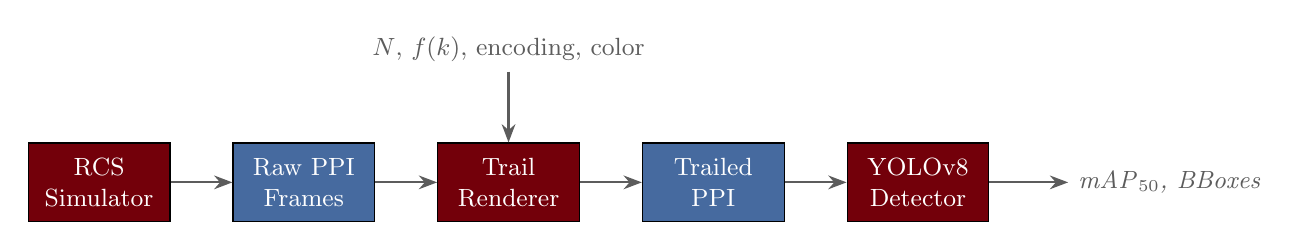
\begin{tikzpicture}[
  box/.style={
    draw,
    rectangle,
    minimum width=1.8cm,
    minimum height=1.0cm,
    align=center,
    font=\small,
    text=white,
    inner sep=4pt,
    rounded corners=0pt
  },
  garnetbox/.style={box, fill=Garnet},
  atlanticbox/.style={box, fill=Atlantic},
  arrow/.style={
    ->,
    >=Stealth,
    thick,
    color=Black70
  }
]

% Nodes
\node[garnetbox]  (rcs)    at (0,0)    {RCS\\Simulator};
\node[atlanticbox](rawppi) at (2.6,0)  {Raw PPI\\Frames};
\node[garnetbox]  (trail)  at (5.2,0)  {Trail\\Renderer};
\node[atlanticbox](tppi)   at (7.8,0)  {Trailed\\PPI};
\node[garnetbox]  (yolo)   at (10.4,0) {YOLOv8\\Detector};

% Arrows between boxes
\draw[arrow] (rcs)    -- (rawppi);
\draw[arrow] (rawppi) -- (trail);
\draw[arrow] (trail)  -- (tppi);
\draw[arrow] (tppi)   -- (yolo);

% Output arrow and label
\draw[arrow] (yolo.east) -- ++(1.0,0)
  node[right, align=left, font=\small, color=Black70]
  {\textit{mAP}$_{50}$\textit{, BBoxes}};

% Annotation arrow pointing down to Trail Renderer
\node[above=0.9cm of trail, align=center, font=\small, color=Black70]
  (annot) {$N$, $f(k)$, encoding, color};
\draw[arrow] (annot.south) -- (trail.north);

\end{tikzpicture}
\end{document}
